\documentclass[tikz,border=5pt]{standalone}
\usepackage{amsmath,lmodern}
\usetikzlibrary{positioning,arrows.meta,fit,backgrounds}
\definecolor{Orange}{HTML}{E69F00}
\definecolor{SkyBlue}{HTML}{56B4E9}
\definecolor{Blue}{HTML}{0072B2}
\definecolor{Vermillion}{HTML}{D55E00}
\definecolor{Purple}{HTML}{CC79A7}
\definecolor{Graphite}{HTML}{4D4D4D}
\begin{document}
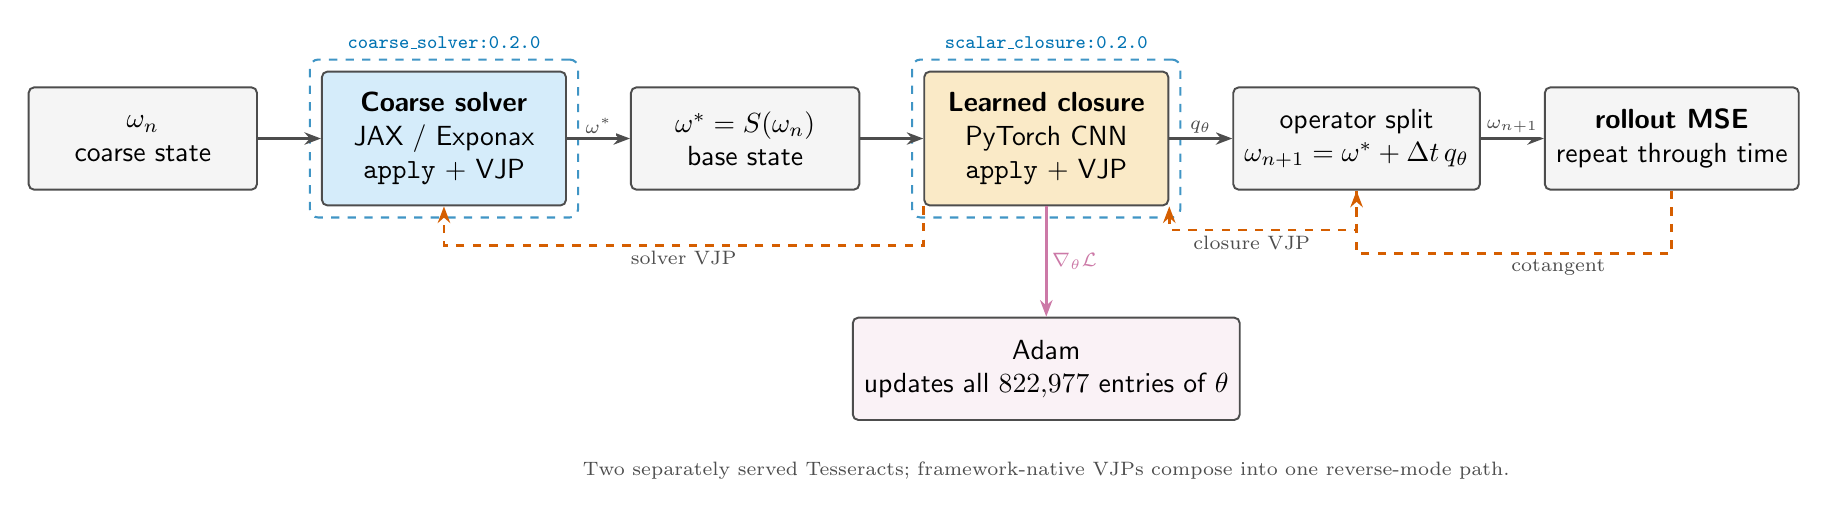
\begin{tikzpicture}[
  font=\sffamily,
  node distance=7mm and 8mm,
  component/.style={rounded corners=2pt,draw=Graphite,line width=.7pt,minimum height=17mm,minimum width=31mm,align=center,inner sep=4pt},
  host/.style={rounded corners=2pt,draw=Graphite,line width=.7pt,fill=black!4,minimum height=13mm,minimum width=29mm,align=center,inner sep=4pt},
  flow/.style={-{Stealth[length=2.1mm]},draw=Graphite,line width=.8pt},
  grad/.style={-{Stealth[length=2.1mm]},draw=Vermillion,dashed,line width=1.05pt},
  update/.style={-{Stealth[length=2.1mm]},draw=Purple,line width=1.05pt},
  edge/.style={font=\scriptsize,fill=white,inner sep=1.5pt,text=Graphite},
  group/.style={rounded corners=3pt,draw=Blue!75,dashed,line width=.75pt,inner sep=4pt},
  grouplabel/.style={font=\scriptsize\bfseries,text=Blue}
]
\node[host] (state) {$\omega_n$\\coarse state};
\node[component,fill=SkyBlue!25,right=of state] (solver) {\textbf{Coarse solver}\\JAX / Exponax\\\texttt{apply} + VJP};
\node[host,right=of solver] (base) {$\omega^*=S(\omega_n)$\\base state};
\node[component,fill=Orange!22,right=of base] (closure) {\textbf{Learned closure}\\PyTorch CNN\\\texttt{apply} + VJP};
\node[host,right=of closure] (split) {operator split\\$\omega_{n+1}=\omega^*+\Delta t\,q_\theta$};
\node[host,right=of split] (loss) {\textbf{rollout MSE}\\repeat through time};
\draw[flow] (state)--(solver);
\draw[flow](solver)--node[edge,above]{$\omega^*$}(base);
\draw[flow](base)--(closure);
\draw[flow](closure)--node[edge,above]{$q_\theta$}(split);
\draw[flow](split)--node[edge,above]{$\omega_{n+1}$}(loss);
\node[host,fill=Purple!10,below=14mm of closure] (adam) {Adam\\updates all $822{,}977$ entries of $\theta$};
\draw[grad](loss.south)--++(0,-8mm)-|node[edge,pos=.18,below]{cotangent}(split.south);
\draw[grad](split.south)--++(0,-5mm)-|node[edge,pos=.28,below]{closure VJP}(closure.south east);
\draw[grad](closure.south west)--++(0,-5mm)-|node[edge,pos=.25,below]{solver VJP}(solver.south);
\draw[update](closure.south)--node[edge,right,text=Purple]{$\nabla_\theta\mathcal L$}(adam.north);
\begin{scope}[on background layer]
  \node[group,fit=(solver),label={[grouplabel]above:\texttt{coarse\_solver:0.2.0}}]{};
  \node[group,fit=(closure),label={[grouplabel]above:\texttt{scalar\_closure:0.2.0}}]{};
\end{scope}
\node[font=\scriptsize,text=Graphite,below=4mm of adam]{Two separately served Tesseracts; framework-native VJPs compose into one reverse-mode path.};
\end{tikzpicture}
\end{document}
